% !TEX root = ../../main.tex

\subsection{Baseline BER Performance Comparison}

After defining the simulation setup, the first performance comparison is made between the conventional OFDM-LMMSE baseline, the baseline OTFS system, and the proposed OTFS-IM schemes. This comparison establishes the main BER trend before the detailed index-modulation analysis is presented. The representative configuration used in this section is \(n=6\), \(k=5\), because it has the same spectral efficiency as the baseline OTFS system:
\begin{equation}
    \eta_{\mathrm{IM}} = \eta_{\mathrm{OTFS}} = 2.00~\mathrm{bits/symbol}.
    \label{eq:chapter5_equal_se_65}
\end{equation}
Therefore, the BER comparison in this section is rate-fair. Any BER improvement of OTFS-IM over OTFS in this configuration is not obtained by reducing the number of transmitted bits per resource element.

\IfFileExists{Images/Chapter5/ber_overview_n6_k5.png}{%
\begin{figure}[H]
    \centering
    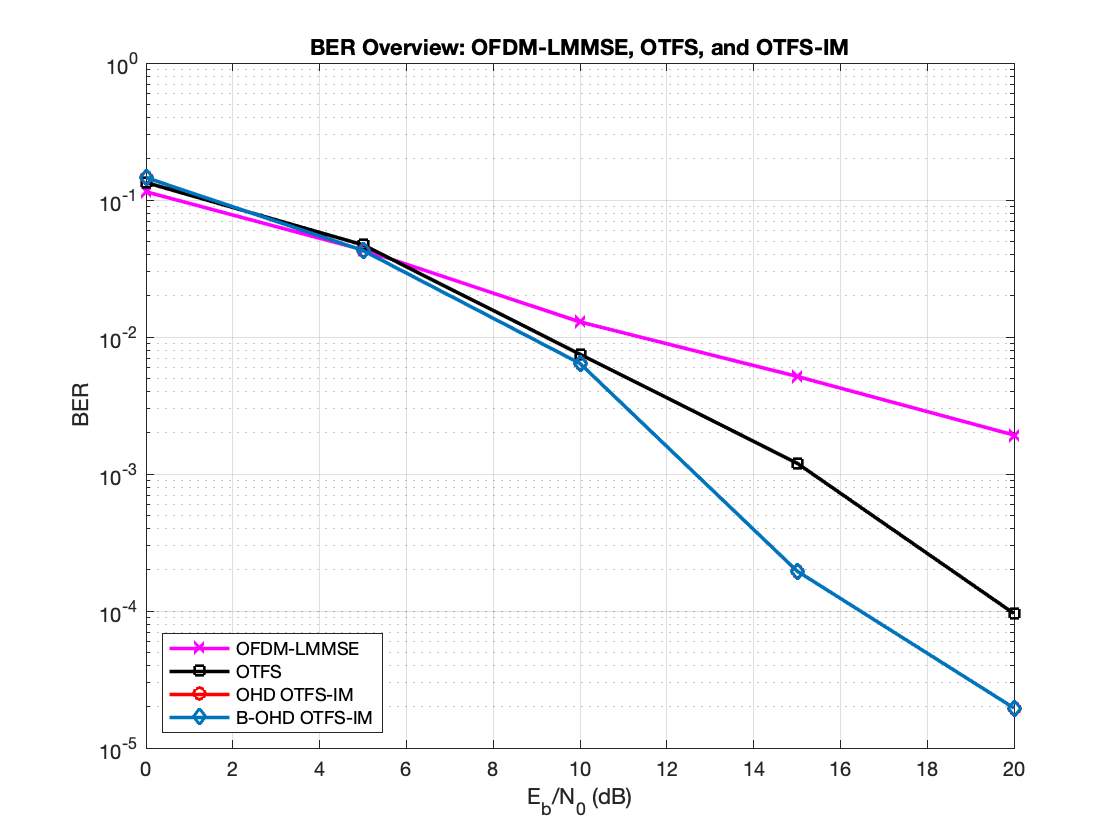
\includegraphics[width=0.88\linewidth]{Images/Chapter5/ber_overview_n6_k5.png}
    \caption{BER overview of OFDM-LMMSE, OTFS, and OTFS-IM for the \(n=6,k=5\) equal-SE configuration}
    \label{fig:chapter5_ber_overview_n6_k5}
\end{figure}
}{%
\begin{figure}[H]
    \centering
    \fbox{\begin{minipage}[c][5cm][c]{0.86\linewidth}
        \centering
        Required figure file is missing:\\
        Images/Chapter5/ber\_overview\_n6\_k5.png
    \end{minipage}}
    \caption{BER overview of OFDM-LMMSE, OTFS, and OTFS-IM for the \(n=6,k=5\) equal-SE configuration}
    \label{fig:chapter5_ber_overview_n6_k5}
\end{figure}
}

Figure~\ref{fig:chapter5_ber_overview_n6_k5} compares the BER of OFDM-LMMSE, baseline OTFS, OHD OTFS-IM, and B-OHD OTFS-IM over the simulated \(E_b/N_0\) range. The OFDM-LMMSE curve is included as the conventional multicarrier reference. Since it uses a full-frame LMMSE equalizer with perfect channel knowledge in the simulation, it should be interpreted as a meaningful OFDM benchmark rather than an unequalized OFDM receiver. The OTFS curve is the main delay-Doppler baseline, while the two OTFS-IM curves show the effect of adding index modulation and deterministic activation-pattern selection.

At low SNR, the BER of all schemes remains relatively high because the receiver is dominated by noise and uncertain symbol probabilities. In this region, the advantage of the delay-Doppler structure is not fully visible, and the additional index-detection task in OTFS-IM may even make the error behavior less stable. This can be observed around \(0\) dB, where the BER of OTFS-IM is not yet better than the baseline schemes. Such behavior is expected because the receiver must simultaneously detect both active positions and QAM symbols.

As the SNR increases, the benefit of OTFS and OTFS-IM becomes clearer. At \(10\) dB, the baseline OTFS BER is approximately \(7.49\times 10^{-3}\), while OHD OTFS-IM and B-OHD OTFS-IM both achieve approximately \(6.41\times 10^{-3}\) for the \(n=6,k=5\) configuration. This indicates a moderate but rate-fair improvement over baseline OTFS. The OFDM-LMMSE BER at the same SNR is approximately \(1.29\times 10^{-2}\), which is higher than the OTFS-based schemes under the same channel conditions.

The difference becomes more pronounced at higher SNR. At \(15\) dB, the baseline OTFS BER is approximately \(1.20\times 10^{-3}\), while OHD and B-OHD OTFS-IM decrease to about \(2.00\times 10^{-4}\). This is the most important region for interpreting the BER overview, because the noise level is low enough for the activation-pattern structure to become useful, but the error rate is still high enough to compare the schemes meaningfully. At \(20\) dB, the OTFS-IM curves approach the Monte Carlo resolution limit of the simulation. Therefore, the \(20\) dB point should be used cautiously and not over-interpreted as an exact zero-error result.

Table~\ref{tab:chapter5_representative_ber_n6_k5} gives the numerical BER values for the representative equal-SE configuration. The table is included to support the visual trend in Figure~\ref{fig:chapter5_ber_overview_n6_k5} and to make the comparison easier to reference in the discussion.

\begin{table}[H]
    \centering
    \caption{Representative BER values for the \(n=6,k=5\) equal-SE configuration}
    \label{tab:chapter5_representative_ber_n6_k5}
    \begin{tabularx}{\linewidth}{>{\centering\arraybackslash}p{2.1cm}
                                  >{\centering\arraybackslash}p{3.0cm}
                                  >{\centering\arraybackslash}p{2.4cm}
                                  >{\centering\arraybackslash}p{2.6cm}
                                  >{\Centering\arraybackslash}X}
        \toprule
        \(E_b/N_0\) (dB) & OFDM-LMMSE BER & OTFS BER & OHD OTFS-IM BER & B-OHD OTFS-IM BER \\
        \midrule
        0  & \(1.1480\times10^{-1}\) & \(1.3407\times10^{-1}\) & \(1.4573\times10^{-1}\) & \(1.4573\times10^{-1}\) \\
        \midrule
        5  & \(4.3280\times10^{-2}\) & \(4.7030\times10^{-2}\) & \(4.2800\times10^{-2}\) & \(4.2800\times10^{-2}\) \\
        \midrule
        10 & \(1.2880\times10^{-2}\) & \(7.4900\times10^{-3}\) & \(6.4100\times10^{-3}\) & \(6.4100\times10^{-3}\) \\
        \midrule
        15 & \(5.1600\times10^{-3}\) & \(1.2000\times10^{-3}\) & \(2.0000\times10^{-4}\) & \(2.0000\times10^{-4}\) \\
        \midrule
        20 & \(1.9300\times10^{-3}\) & \(1.0000\times10^{-4}\) & \(0\) & \(0\) \\
        \bottomrule
    \end{tabularx}
\end{table}

The table also shows that OHD and B-OHD have identical BER values in this configuration. This happens because the selected activation-pattern tables are effectively the same for \(n=6,k=5\). Since the valid pattern space is highly constrained in this case, the additional balancing criteria of B-OHD do not change the final selected pattern set. This observation is important for the following sections: B-OHD should not be expected to outperform OHD in every configuration. Its value becomes clearer only when the pattern space is large enough for the balance criterion to alter the selected table.

To illustrate a configuration where OHD and B-OHD do not completely overlap, Figure~\ref{fig:chapter5_ber_overview_n5_k3} shows the BER overview for \(n=5,k=3\). Unlike the previous equal-SE case, this configuration has
\begin{equation}
    \eta_{\mathrm{IM}} = 1.80~\mathrm{bits/symbol},
    \label{eq:chapter5_se_53}
\end{equation}
which is lower than the baseline OTFS spectral efficiency. Therefore, the \(n=5,k=3\) result should be interpreted as a reliability-rate trade-off rather than a direct rate-fair improvement.

\IfFileExists{Images/Chapter5/ber_overview_n5_k3.png}{%
\begin{figure}[H]
    \centering
    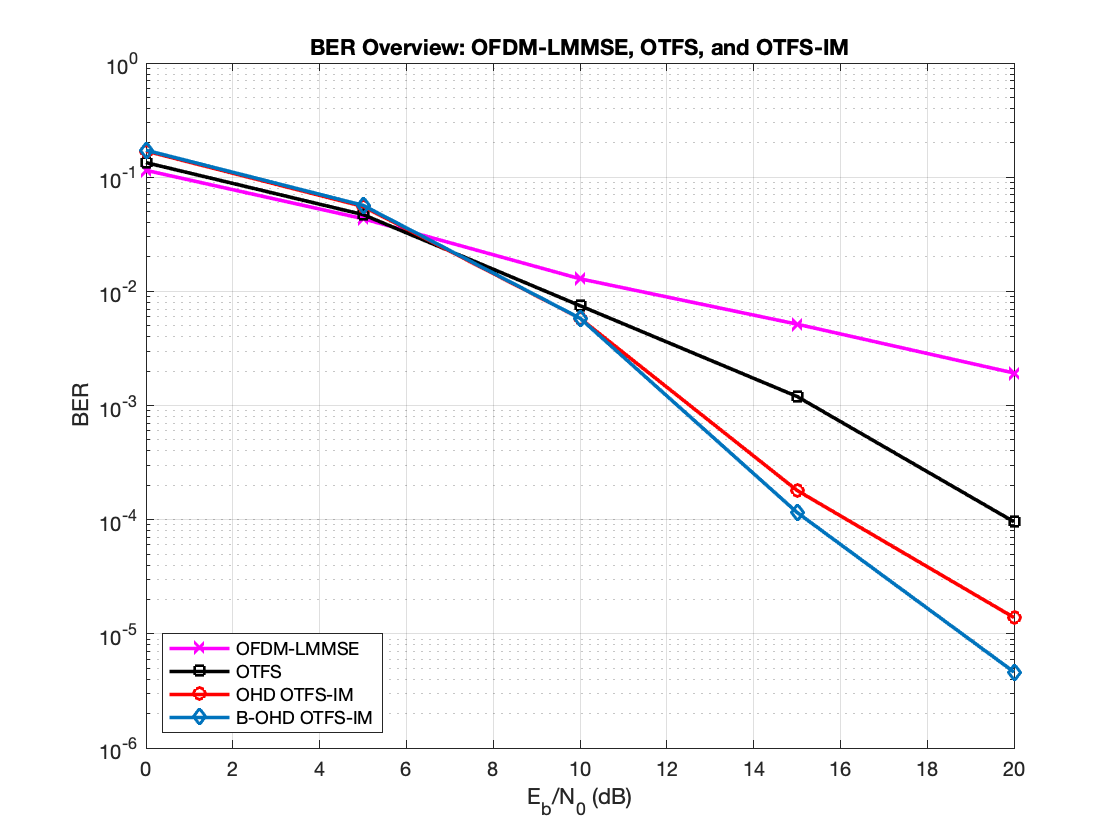
\includegraphics[width=0.88\linewidth]{Images/Chapter5/ber_overview_n5_k3.png}
    \caption{BER overview of OFDM-LMMSE, OTFS, and OTFS-IM for the \(n=5,k=3\) trade-off configuration}
    \label{fig:chapter5_ber_overview_n5_k3}
\end{figure}
}{%
\begin{figure}[H]
    \centering
    \fbox{\begin{minipage}[c][5cm][c]{0.86\linewidth}
        \centering
        Required figure file is missing:\\
        Images/Chapter5/ber\_overview\_n5\_k3.png
    \end{minipage}}
    \caption{BER overview of OFDM-LMMSE, OTFS, and OTFS-IM for the \(n=5,k=3\) trade-off configuration}
    \label{fig:chapter5_ber_overview_n5_k3}
\end{figure}
}

For \(n=5,k=3\), OHD and B-OHD no longer represent the same selected table. At \(10\) dB, both deterministic OTFS-IM schemes achieve approximately \(5.81\times10^{-3}\), which is lower than the baseline OTFS BER of approximately \(7.49\times10^{-3}\). At \(15\) dB, B-OHD becomes better than OHD, with a BER of about \(1.16\times10^{-4}\) compared with \(1.81\times10^{-4}\) for OHD. This behavior shows that the balancing criterion can change the high-SNR error trend, but the result must still be interpreted as a reliability-rate trade-off because \(\eta_{\mathrm{IM}}<\eta_{\mathrm{OTFS}}\). This configuration is therefore useful for pattern-selection analysis, while the \(n=6,k=5\) case remains the main rate-fair BER evidence.

Overall, this baseline comparison shows three important trends. First, OTFS-based transmission becomes more reliable than OFDM-LMMSE as the SNR increases under the considered delay-Doppler channel. Second, OTFS-IM can improve BER over baseline OTFS while maintaining the same spectral efficiency in the representative \(n=6,k=5\) case. Third, when the pattern table changes as in \(n=5,k=3\), OHD and B-OHD can produce different BER behavior, but the result must be interpreted together with spectral efficiency. For this reason, the next section focuses specifically on equal-spectral-efficiency OTFS-IM configurations before moving to pattern-level error analysis.
